\documentclass[12pt,a4paper]{article}
\usepackage[utf8]{inputenc}
\usepackage[russian]{babel}
\usepackage[OT1]{fontenc}
\usepackage{mathtools}
\usepackage{amsfonts}
\usepackage{amssymb}
\usepackage{enumitem}
\usepackage{alltt}
\usepackage{graphicx}
\usepackage{indentfirst}
\usepackage{caption}
\usepackage{float}
\usepackage{wrapfig}
\usepackage{physics}
\usepackage{multirow}
\usepackage{longtable}
\usepackage{amsmath,amsfonts,amssymb,amsthm,mathtools}
\usepackage{icomma}
\setlength{\parindent}{0.75cm}
\graphicspath{{pictures/}}
\DeclareGraphicsExtensions{.png}
\usepackage[left=15mm,right=15mm,top=2cm,bottom=2cm]{geometry}
\author{Глотов Алексей}
\begin{document}
\newpage
\begin{center}
\footnotesize{{ГОСУДАРСТВЕННОЕ АВТОНОМНОЕ ОБРАЗОВАТЕЛЬНОЕ УЧРЕЖДЕНИЕ}\break
{ВЫСШЕГО ОБРАЗОВАНИЯ}
\break
{\bf {МОСКОВСКИЙ ФИЗИКО-ТЕХНИЧЕСКИЙ ИНСТИТУТ}}
\break
\small{(НАЦИОНАЛЬНЫЙ ИССЛЕДОВАТЕЛЬСКИЙ УНИВЕРСИТЕТ)}}
\break
\hfill \break
\hfill \break
\begin{center}
\normalsize{Кафедра общей физики}
\end{center}
\hfill \break
\hfill \break
\hfill \break
\hfill \break

\begin{center}
\normalsize {Лабораторная работа 2.1.3}
\end{center}
\hfill \break\\
\large{\textbf{Определение $C_{p}/C_{v}$ по скорости звука в газе}}
\end{center}
\begin{flushleft}
\hfill \break
\hfill \break
\hfill \break
\hfill \break
\hfill \break
\hfill \break
\hfill \break
\hfill \break
\hfill \break
\hfill \break
\hangindent=9cm
\normalsize{Преподаватель:}\hfill
\normalsize{доцент Игуманов А.Ю.}\\
\hfill \break
\normalsize{Обучающийся:}\hfill
\normalsize{Глотов А.А} \\
\hfill \break
\end{flushleft}
\hfill \break
\hfill \break
\hfill \break
\hfill \break
\hfill \break
\hfill \break
\hfill \break
\hfill \break
\hfill \break
\hfill \break
\hfill \break

\begin{center}
Долгопрудный \break
 2022
\end{center}
\thispagestyle{empty}
\section{Введение}
\subsection{Аннотация}

Данная работа посвящена изучению резонанса звуковой волны в газах. Используются следующие методы измерений: анализ и линеаризация графиков зависимостей $\Delta{L}(k)$ и $f(k)$. Настройка установок производится вручную и с использованием электронных приборов

\textbf{Цель работы:}  \begin{enumerate}
\item измерение частоты колебаний и длины волны при резонансе звуковых колебаний в газе, заполняющем трубу;
\item определение показателя адиабаты с помощью уравнения состояния идеального газа.
\end{enumerate}

\textbf{В работе используются:} звуковой генератор ГЗ; электронный осциллограф ЭО; микрофон; телефон; раздвижная труба; теплоизолированная труба, обогреваемая водой из термостата; баллон со сжатым углекислым газом; газгольдер.

\subsection{Теоретические сведения}

Скорость распространения звуковой волны в газах зависит от показателя адиабаты $ \gamma $. На измерении скорости звука основан один из наиболее точных методов определения показателя адиабаты.

Скорость звука в газах определяется формулой:

\begin{equation}\label{velocity}
c=\sqrt{\gamma\frac{RT}{\mu}}.
\end{equation}
где $ R $ -- газовая постоянная, $ T $ -- температура газа, а $ \mu $ -- его молярная масса. Преобразуя эту формулу, найдем
\begin{equation}\label{gamma}
\boxed{\gamma = \frac{\mu}{RT}c^2}.
\end{equation}

Таким образом, для определения показателя адиабаты достаточно измерить температуру газа и скорость распространения звука (молярная масса газа предполагается известной).

Звуковая волна, распространяющаяся вдоль трубы, испытывает многократные отражения от торцов. Звуковые колебания в трубе являются наложением всех отраженных волн и очень сложны. Картина упрощается, если длина трубы $ L $ равна целому числу полуволн, то есть когда \[ L=n\lambda/2, \] где $ \lambda $ -- длина волны звука в трубе, а $ n $ -- любое целое число. Если это условие выполнено, то волна, отраженная от торца трубы, вернувшаяся к ее началу и вновь отраженная, совпадает по фазе с падающей. Совпадающие по фазе волны усиливают друг друга. Амплитуда звуковых колебаний при этом резко возрастает -- наступает резонанс.

При звуковых колебаниях слои газа, прилегающие к торцам трубы, не испытывают смещения. Узлы смещения повторяются по всей длине трубы через $ \lambda/2 $. Между узлами находятся максимумы смещения.

Скорость звука c связана с его частотой $ f $ и длиной волны $ \lambda $ соотношением

\begin{equation}\label{lambda_f}
c=\lambda f.
\end{equation}

\subsection{Схема эксперимента}

Соответственно двум методам измерения скорости звука в работе имеются две установки (рис. \ref{img1} и \ref{img2}). В обеих установках звуковые колебания в трубе возбуждаются телефоном Т и улавливаются микрофоном М. Мембрана телефона приводится в движение переменным током звуковой частоты; в качестве источника переменной ЭДС используется звуковой генератор ГЗ. Возникающий в микрофоне сигнал наблюдается на осциллографе ЭО.

Микрофон и телефон присоединены к установке через тонкие резиновые трубки. Такая связь достаточна для возбуждения и обнаружения звуковых колебаний в трубе и в то же время мало возмущает эти колебания: при расчетах оба торца трубы можно считать неподвижными, а влиянием соединительных отверстий пренебречь.

\subsection{Методика измерений}

Подбор условий, при которых возникает резонанс, можно производить двояко:
\begin{enumerate}
	\item При неизменной частоте $ f $ звукового генератора (а следовательно, и неизменной длине звуковой волны $ \lambda $) можно изменять длину трубы $ L $. Для этого применяется раздвижная труба. Длина раздвижной трубы постепенно увеличивается, и наблюдается ряд последовательных резонансов. Возникновение резонанса легко наблюдать на осциллографе по резкому увеличению амплитуды колебаний. Для последовательных резонансов имеем \begin{equation}\label{first}
	L_n=n\frac{\lambda}{2}, \quad L_{n+1}=(n+1)\frac{\lambda}{2}, \quad \dots, \quad L_{n+k} = n\frac{\lambda}{2}+k\frac{\lambda}{2},
	\end{equation} т. е. $ \lambda/2 $ равно угловому коэффициенту графика, изображающего зависимость длины трубы $ L $ от номера резонанса $ k $. Скорость звука находится по формуле \eqref{lambda_f}.
	\item При постоянной длине трубы можно изменять частоту звуковых колебаний. В этом случае следует плавно изменять частоту $ f $ звукового генератора, а следовательно, и длину звуковой волны $ \lambda $. Для последовательных резонансов получим 
	\begin{equation}\label{4}
	L=\frac{\lambda_1}{2}n=\frac{\lambda_2}{2}(n+1)=\dots=\frac{\lambda_{k+1}}{2}(n+k).
	\end{equation}
	
	Из \eqref{lambda_f} и \eqref{4} имеем:
	\[ f_1=\frac{c}{\lambda_1}=\frac{c}{2L}n, \quad f_2=\frac{c}{\lambda_2}=\frac{c}{2L}(n+1)=f_1+\frac{c}{2L},\quad \dots, \]
	\begin{equation}\label{5}
	f_{k+1}=\frac{c}{\lambda_{k+1}}=\frac{c}{2L}(n+k)=f_1+\frac{c}{2L}k.
	\end{equation}
	Скорость звука, деленная на $ 2L $, определяется, таким образом, по угловому коэффициенту графика зависимости частоты от номера резонанса.
\end{enumerate}


\subsection{Экспериментальная установка}

Первая установка (рис. \ref{img1}) содержит раздвижную трубу с миллиметровой шкалой. Через патрубок (на рисунке не показан) труба может наполняться воздухом или углекислым газом из газгольдера. На этой установке производятся измерения $ \gamma $ для воздуха и для $ CO_2 $. Вторая установка (рис. \ref{img2}) содержит теплоизолированную трубу постоянной длины. Воздух в трубе нагревается водой из термостата. Температура газа принимается равной температуре омывающей трубу воды. На этой установке измеряется зависимость скорости звука от температуры.

\begin{figure}[H]
	\begin{center}
		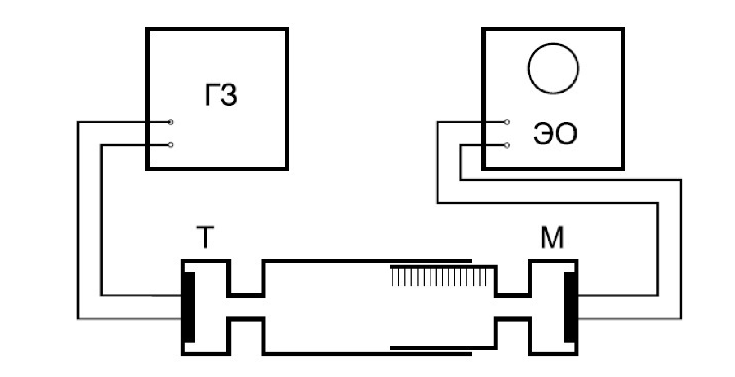
\includegraphics[width=12cm]{2.1.3_1}
	\end{center}
	\caption{\textit{Установка для измерения скорости звука при помощи раздвижной трубы}}
	\label{img1}
\end{figure}

\begin{figure}[H]
	\begin{center}
		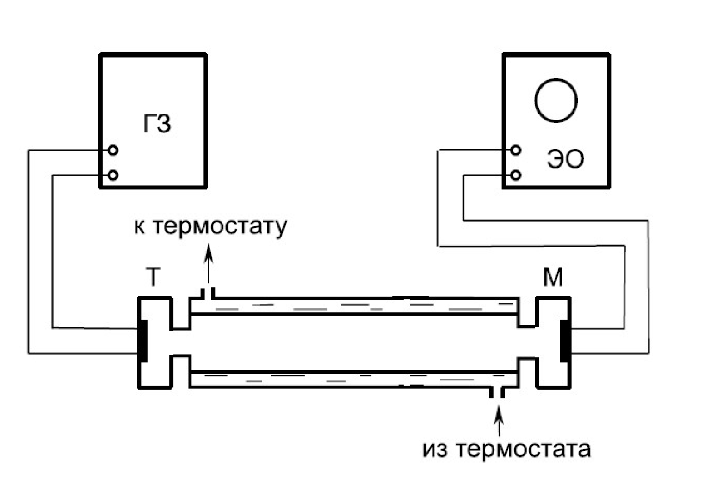
\includegraphics[width=12cm]{2.1.3_2}
	\end{center}
	\caption{\textit{Установка для изучения зависимости скорости звука от температуры}}
	\label{img2}
\end{figure}

\newpage

\section{Результаты измерений и обработка данных}

\subsection{Измерения при переменной длине трубы}
\subsection*{Измерения скорости звука в воздухе}
Зафиксируем параметры нашей системы: \hfill \break 
$L_{0} = (570 \pm 5)$ мм - начальная длина трубы \hfill \break 
$T = 293.4$К - температура окружающей среды 

Проведем несколько серий измерений, изменяя частоту звуковых колебаний. Отследим и зафиксируем точки, когда наблюдается эффект резонанса. Занесем результаты измерений в таблицу
\begin{center}

\begin{tabular}{|p{0.25\textwidth}|p{0.1\textwidth}|p{0.1\textwidth}|p{0.1\textwidth}|p{0.1\textwidth}|p{0.1\textwidth}|p{0.1\textwidth}|p{0.1\textwidth}|}
\hline 
k & 1  & 2 & 3 & 4 & 5 & 6 \\ 
\hline 
\multicolumn{7}{|c|}{f = 3.5 кГц} \\ 
\hline 
$\Delta{L_{forward}}$, мм  & 26 & 75 & 125 & 174 & 223 & - \\ 
\hline 
$\Delta{L_{back}}$, мм  & 26 & 76 & 125 & 175 & - & - \\ 
\hline 
\multicolumn{7}{|c|}{f = 4.0 кГц} \\ 
\hline 
$\Delta{L_{forward}}$, мм  & 40 & 83 & 127 & 169 & 213 & - \\ 
\hline 
$\Delta{L_{back}}$, мм  & 40 & 82 & 126 & 170 & - & - \\ 
\hline 
\multicolumn{7}{|c|}{f = 4.5 кГц} \\ 
\hline 
$\Delta{L_{forward}}$, мм  & 11 & 48 & 87 & 126 & 164 & 202 \\ 
\hline 
$\Delta{L_{back}}$, мм  & 11 & 49 & 87 & 126 & 164 & - \\ 
\hline 
\multicolumn{7}{|c|}{f = 5.0 кГц} \\ 
\hline 
$\Delta{L_{forward}}$, мм  & 22 & 57 & 92 & 127 & 161 & 196 \\ 
\hline 
$\Delta{L_{back}}$, мм  & 21 & 57 & 91 & 126 & 160 & - \\ 
\hline 
\multicolumn{7}{|c|}{f = 5.5 кГц} \\ 
\hline 
$\Delta{L_{forward}}$, мм  & 32 & 65 & 96 & 127 & 159 & 191 \\ 
\hline 
$\Delta{L_{back}}$, мм  & 32 & 65 & 96 & 127 & 160 & - \\ 
\hline 
\multicolumn{7}{|c|}{f = 6.0 кГц} \\ 
\hline 
$\Delta{L_{forward}}$, мм  & 13 & 41 & 71 & 100 & 128 & 151 \\ 
\hline 
$\Delta{L_{back}}$, мм  & 13 & 41 & 71 & 99 & 127 & - \\ 
\hline 
\end{tabular} 
\end{center}
$\sigma{L} = 1$ мм

По данным из таблицы построим графики зависимости $\Delta{L}(k)$. Перед этим необходимо отметить, что ввиду незначительного (в пределах приборной погрешности) отличия значений при проходе в разные стороны, будем считать их одинаковыми


\begin{figure}[H]
	\begin{center}
		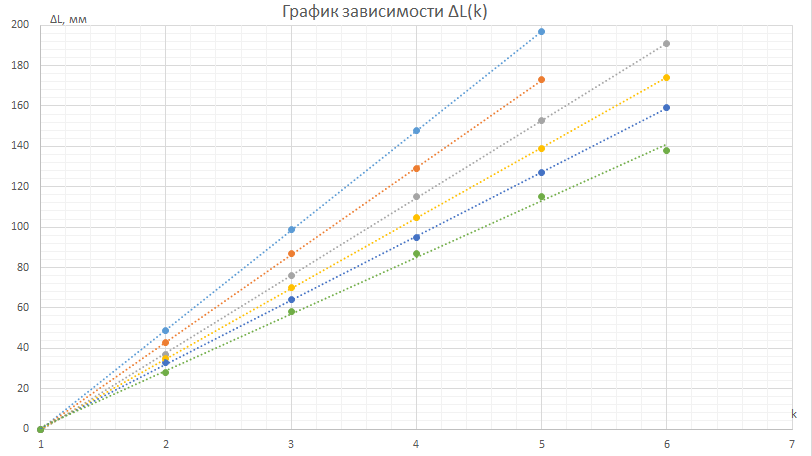
\includegraphics[width=14cm]{2.1.3_gr_1}
	\end{center}
\end{figure}

Определим угловые коэффициенты наших прямых

$\frac{\lambda}{2}=\alpha=\frac{<k\Delta{L}>-<\Delta{L}><k>}{<k^2>-<k>^2}$ \;\;\;\;\;\;\; $\sigma_{\alpha}=\sqrt{\frac{1}{N-2}(\frac{<{\Delta{L}}^2>-<\Delta{L}>^2}{<k^2>-<k^2}-{\alpha}^2)}$

$\varepsilon_{\lambda} = \varepsilon_{\alpha} = \varepsilon_{c}$ (ввиду малости погрешности f)

Для наглядности сдвинем наши прямые к одной точки, вычитая из каждого измерения значение первого для данной серии значений. Заранее оговорим, что эти графики не используются в дальнейшем для анализа из-за увеличивающейся погрешности

Определим значения угловых коэффициентов наших прямых, а после - значения скоростей звука. Систематическую (в данной работе - приборную), возьмем как усредненную погрешность для всех $\Delta{L}$ в серии измерений

С помощью (3) посчитаем значение скорости звука. Из нее напрямую следует, что $\sigma_{c} = c\frac{\sigma_{\lambda}}{\lambda}$

\begin{center}
\begin{tabular}{|c|c|c|c|c|c|c|}
 \hline 
 f, кГц & $\lambda$, мм & $\sigma^{\text{случ}}{\lambda}$, мм & $\sigma^{\text{сист}}{\lambda}$, мм & $\sigma{\lambda}$, мм & c, $\frac{\text{м}}{c}$ & $\sigma{c}, \frac{\text{м}}{c}$ \\ 
 \hline 
 3.5 & 98.6 & 0.2 & 1.4 & 1.4 & 345.1 & 4.9 \\ 
 \hline 
 4.0 & 86.4 & 0.3 & 1.0 & 1.0 & 345.6 & 4 \\ 
 \hline 
 4.5 & 76.7 & 0.3 & 1.8 & 1.8 & 345.2 & 8.1 \\ 
 \hline 
 5.0 & 69.5 & 0.1 & 1.1 & 1.1 & 347.5 & 5.5 \\ 
 \hline 
 5.5 & 63.3 & 0.3 & 0.8 & 0.8 & 348.2 & 4.4 \\ 
 \hline 
 6.0 & 56.0 & 1.0 & 1.3 & 1.6 & 336.0 & 9.6 \\ 
 \hline 
 \end{tabular}  
\end{center}

Аналогично предыдущему пункту, посчитаем все значения c и их погрешности

Видно, что значения полученные для скорости звука в воздухе, различаются, однако укладываются в пределы нашей погрешности измерений. Для дальнейших действий посчитаем среднее значение из полученных.

$c_{\text{в}} = (344.6 \pm 5.8)\frac{\text{м}}{c}$ 

\subsection*{Измерения скорости звука в углекислом газе}

Проведем аналогичные измерения и обработку данных для углекислого газа

\begin{center}

\begin{tabular}{|p{0.25\textwidth}|p{0.1\textwidth}|p{0.1\textwidth}|p{0.1\textwidth}|p{0.1\textwidth}|p{0.1\textwidth}|p{0.1\textwidth}|p{0.1\textwidth}|}
\hline 
k & 1  & 2 & 3 & 4 & 5 & 6 \\ 
\hline 
\multicolumn{7}{|c|}{f = 5.0 кГц} \\ 
\hline 
$\Delta{L_{forward}}$, мм  & 10 & 41 & 70 & 97 & 126 & - \\ 
\hline 
$\Delta{L_{back}}$, мм  & 18 & 46 & 74 & 102 & - & - \\ 
\hline 
\multicolumn{7}{|c|}{f = 4.5 кГц} \\ 
\hline 
$\Delta{L_{forward}}$, мм  & 22 & 56 & 90 & 123 & 162 & - \\ 
\hline 
$\Delta{L_{back}}$, мм  & 32 & 63 & 90 & 126 & - & - \\ 
\hline 
\multicolumn{7}{|c|}{f = 4.0 кГц} \\ 
\hline 
$\Delta{L_{forward}}$, мм  & - & 46 & 80 & 124 & 157 & 204 \\ 
\hline 
$\Delta{L_{back}}$, мм  & 17 & 52 & 90 & 126 & 161 & - \\ 
\hline 
\multicolumn{7}{|c|}{f = 3.5 кГц} \\ 
\hline 
$\Delta{L_{forward}}$, мм  & 24 & 62 & 105 & 150 & 195 & - \\ 
\hline 
$\Delta{L_{back}}$, мм  & 28 & 72 & 113 & 154 & - & - \\ 
\hline 
\end{tabular} 
\end{center}

В этой части наблюдается заметное расхождение точек при использовании для построения графика точек из "прямого прохода" и усредненных, и при этом относительно небольшое - при использовании точек "обратного прохода". Это несложно объяснить тем, что углекислый газ не успевает при первом проходе заполнить трубу полностью. В связи с этим, для анализа будут использоваться точки "обратного прохода".

\begin{figure}[H]
	\begin{center}
		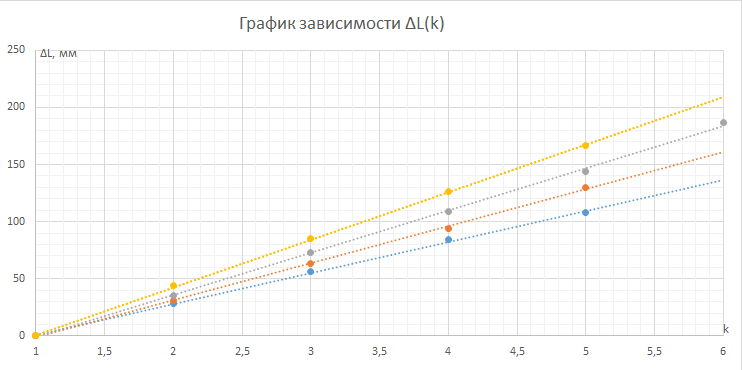
\includegraphics[width=14cm]{2.1.3_gr_2}
	\end{center}
\end{figure}

\begin{center}
\begin{tabular}{|c|c|c|c|c|c|c|}
 \hline 
 f, кГц & $\lambda$, мм & $\sigma^{\text{случ}}{\lambda}$, мм & $\sigma^{\text{сист}}{\lambda}$, мм & $\sigma{\lambda}$, мм & c, $\frac{\text{м}}{c}$ & $\sigma{c}, \frac{\text{м}}{c}$ \\ 
 \hline 
 3.5 & 83.2 & 0.5 & 0.9 & 1.0 & 291.2 & 3.5 \\ 
 \hline 
 4.0 & 74.2 & 0.5 & 1.3 & 1.4 & 296.8 & 5.6 \\ 
 \hline 
 4.5 & 64.6 & 0.5 & 1.3 & 1.4 & 290.7 & 6.3 \\ 
 \hline 
 5.0 & 54.4 & 0.3 & 2.1 & 2.1 & 272.0 & 10.5 \\ 
 \hline 
 \end{tabular}  
\end{center}

$c_{CO_{2}} = (287.7 \pm 6.5)\frac{\text{м}}{c}$

\subsection{Измерения при переменной температуре системы}

Проведем аналогичные измерения на установке, в этот раз меняя температуру системы и снимая резонансные частоты.

Запишем характеристики установки:

$L = (800 \pm 1)$ мм

\begin{center}

\begin{tabular}{|p{0.15\textwidth}|p{0.15\textwidth}|p{0.15\textwidth}|p{0.15\textwidth}|p{0.15\textwidth}|p{0.15\textwidth}|}
\hline 
k & 1  & 2 & 3 & 4 & 5 \\ 
\hline 
\multicolumn{6}{|c|}{T = 295.0 K} \\ 
\hline 
f, Гц  & 200 & 450 & 660 & 872 & 1086 \\ 
\hline 
f, Гц  & 200 & 450 & 660 & 872 & - \\ 
\hline 
\multicolumn{6}{|c|}{T = 300.8 K} \\ 
\hline 
f, Гц  & 200 & 451 & 662 & 878 & 1099 \\ 
\hline 
f, Гц  & 200 & 452 & 662 & 877 & -  \\ 
\hline 
\multicolumn{6}{|c|}{T = 306.6 K} \\ 
\hline 
f, Гц  & 203 & 454 & 667 & 883 & 1100 \\ 
\hline 
f, Гц  & 204 & 454 & 667 & 885 & - \\ 
\hline 
\multicolumn{6}{|c|}{T = 310.0 K} \\ 
\hline 
f, Гц  & 204 & 457 & 671 & 889 & 1107 \\ 
\hline 
f, Гц  & 204 & 457 & 670 & 889 & - \\ 
\hline 
\multicolumn{6}{|c|}{T = 315 K} \\ 
\hline 
f, Гц  & 203 & 459 & 675 & 894 & 1114 \\ 
\hline 
f, Гц  & 206 & 459 & 675 & 894 & - \\ 
\hline 
\multicolumn{6}{|c|}{T = 320.5 K} \\ 
\hline 
f, Гц  & 207 & 463 & 680 & 900 & 1121 \\ 
\hline 
f, Гц  & 207 & 463 & 681 & 900 & - \\ 
\hline 
\multicolumn{6}{|c|}{T = 325.0 K} \\ 
\hline 
f, Гц  & 210 & 465 & 684 & 905 & 1128  \\ 
\hline 
f, Гц  & 209 & 465 & 684 & 906 & -\\ 
\hline 
\end{tabular} 
\end{center}

\begin{figure}[H]
	\begin{center}
		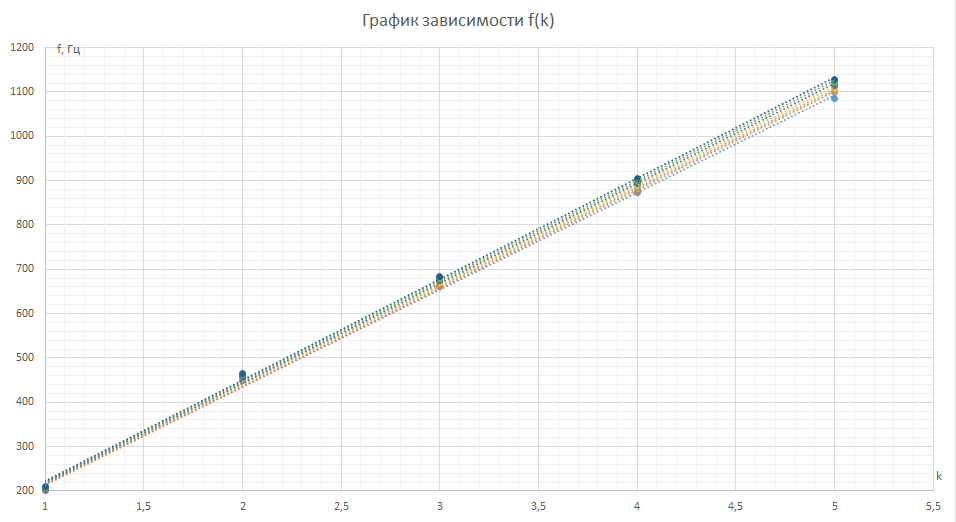
\includegraphics[width=14cm]{2.1.3_gr_3}
	\end{center}
\end{figure}

Аналогично предыдущим пунктам, получим значения углоых коэффициентов и их погрешности. Запишем полученные результаты в таблицу и пересчитаем наши угловые коэффициенты в скорость звука.

Ввиду малости систематических погрешностей, будем считать, что погрешность скорости звука определяется только случайной погрешностью.

\begin{center}
\begin{tabular}{|c|c|c|c|c|}
 \hline 
 T, K & k, Гц & $\sigma_{k}$, Гц &  c, $\frac{\text{м}}{c}$ & $\sigma{c}, \frac{\text{м}}{c}$ \\ 
 \hline 
 295.0 & 219.4 & 4.3 & 351.0 & 6.9  \\ 
 \hline 
 300.8 & 222.5 & 3.9 & 356.0 & 6.2  \\ 
 \hline 
 306.6 & 222.3 & 4.0 & 355.7 & 6.4  \\ 
 \hline 
 310.0 & 223.8 & 4.1 & 358.1 & 6.6  \\ 
 \hline 
 315.0 & 225.7 & 4.2 & 361.1 & 6.7  \\ 
 \hline 
 320.5 & 226.5 & 4.1 & 362.4 & 6.6  \\ 
 \hline 
 325.0 & 227.6 & 3.8 & 364.2 & 6.1  \\ 
 \hline 
 \end{tabular}  
\end{center}

\subsection{Вычисление значения $C_{p}/C_{v}$}

По формуле (2) посчитаем значения $\gamma$ для воздуха по результатам каждого из двух экспериментов

$\mu = 29 \frac{\text{г}}{\text{моль}}$ 

$\sigma_{\gamma} = 2\gamma\frac{\sigma_{c}}{c}$ 

Остальными погрешностями пренебрежем ввиду их малости

$\gamma_{L} = \frac{\mu}{RT}c^2 = 1.41$

$\sigma_{gamma} = 0.05$, $\varepsilon_{\gamma} = 3 \%$

$\gamma_{T} = \frac{\mu}{RT}c^2 = 1.46$

$\sigma_{gamma} = 0.06$, $\varepsilon_{\gamma} = 4 \%$

\newpage

\section{Обсуждение результатов и выводы}

В ходе работы были достигнуты следующие цели:
\begin{itemize}
\item Зафиксировано явление резонанса звуковой волны при изменении частоты колебаний и длины трубы, а также при переменной температуре
\item Зафиксированы изменения в эксперименте при использовании воздуха и углекислого газа
\item Определён показатель адиабаты воздуха как идеального газа, а также скорости звука в воздухе и углекислом газе
\end{itemize}


Для первой серии экспериментов значение показателя адиабаты $1,41 \pm 0.05$ получено с точностью 3\%, причем основной вклад внесли систематические погрешности (изменения длины трубы), что говорит о возможности увеличения точности, если увеличить точность приборов, используемых для измерения длины.

Для второй серии экспериментов значение показателя адиабаты $1,46 \pm 0.06$ получено с точностью 4\%, причем основной вклад внесли случайные погрешности, что говорит о принципиальной невозможности увеличения точности на используемой установке.

Табличное значение равно $1.4$, что с хорошей точностью совпадает с полученным в первой серии экспериментов и лежит в пределах погрешности значения, полученного во второй серии экспериментов. Таким образом, можно утверждать, что приемлемый результат дают оба метода, однако значительно более точным является использование переменной длины. Наиболее вероятно, что это связано с возможностью повторения эксперимента на других частотах и дальнейшего усреднения полученных результатов, что значительно увеличивает вероятность получения истинных значений.

Значения скорости звука в воздухе $(344.6 \pm 5.8) \frac{\text{м}}{c}$ и $(351.0 \ pm 6.9) \frac{\text{м}}{c}$ получены с погрешностями 2\% (1 и 2 серии экспериментов соответственно). Табличное значение при наших условиях составляет примерно $343 \frac{\text{м}}{c}$. Это опять же говорит о лучшей точности первого метода. Значение скорости звука в углекислом газе равно $(287 \pm 6,5) \frac{\text{м}}{c}$ с точностью 2\%. Табличное значение равно $261 \frac{\text{м}}{c}$. Заметное отклонение и непопадание в наши ворота, вероятнее всего, говорит о плохой накачке трубы углекислым газом, а также наличии воздуха (смещение значения скорости в сторону скорости звука в воздухе). Однако полученное значение можно считать приемлемым.

Также нами была проведена серия экспериментов с изменением температуры системы. Несмотря на малость изменений, можно однозначно утверждать о тенденции роста скорости звука в воздухе с ростом температуры, что качественно соответствует теоретическим выкладкам 

\end{document}